\section{Kết quả GRNR}

\begin{frame}{GRNR tại $d=1$: Chưa phân biệt được với EASE đầy đủ}
\centering
\small
\begin{tabular}{lrr}
\toprule
\textbf{Nhóm giải trực tiếp (test)} & \textbf{NDCG@20} $\uparrow$ & \textbf{Recall@20} $\uparrow$\\
\midrule
\rowcolor{PaleBlue}\textbf{GRNR} & \textbf{0,02843} & \textbf{0,05941}\\
EASE đầy đủ & 0,02809 & 0,05834\\
EASE top-128 & 0,02635 & 0,05312\\
GF-CF & 0,01280 & 0,02835\\
\bottomrule
\end{tabular}
\vspace{0.38cm}
\begin{block}{Kiểm định NDCG@20}
\small
GRNR $-$ EASE đầy đủ: $+0{,}00034$; KTC 95\% $[-0{,}00003;\,+0{,}00072]$.\\[5pt]
GRNR $-$ EASE top-128: $+0{,}00209$; KTC 95\% $[+0{,}00174;\,+0{,}00247]$.
\end{block}
\vspace{0.22cm}
\takeaway{Có lợi thế so với \textbf{EASE top-128 cùng giới hạn hệ số}; chưa đủ bằng chứng vượt EASE đầy đủ.}
\end{frame}

\begin{frame}{GRNR theo $d$: So với EASE và MostPop}
\centering
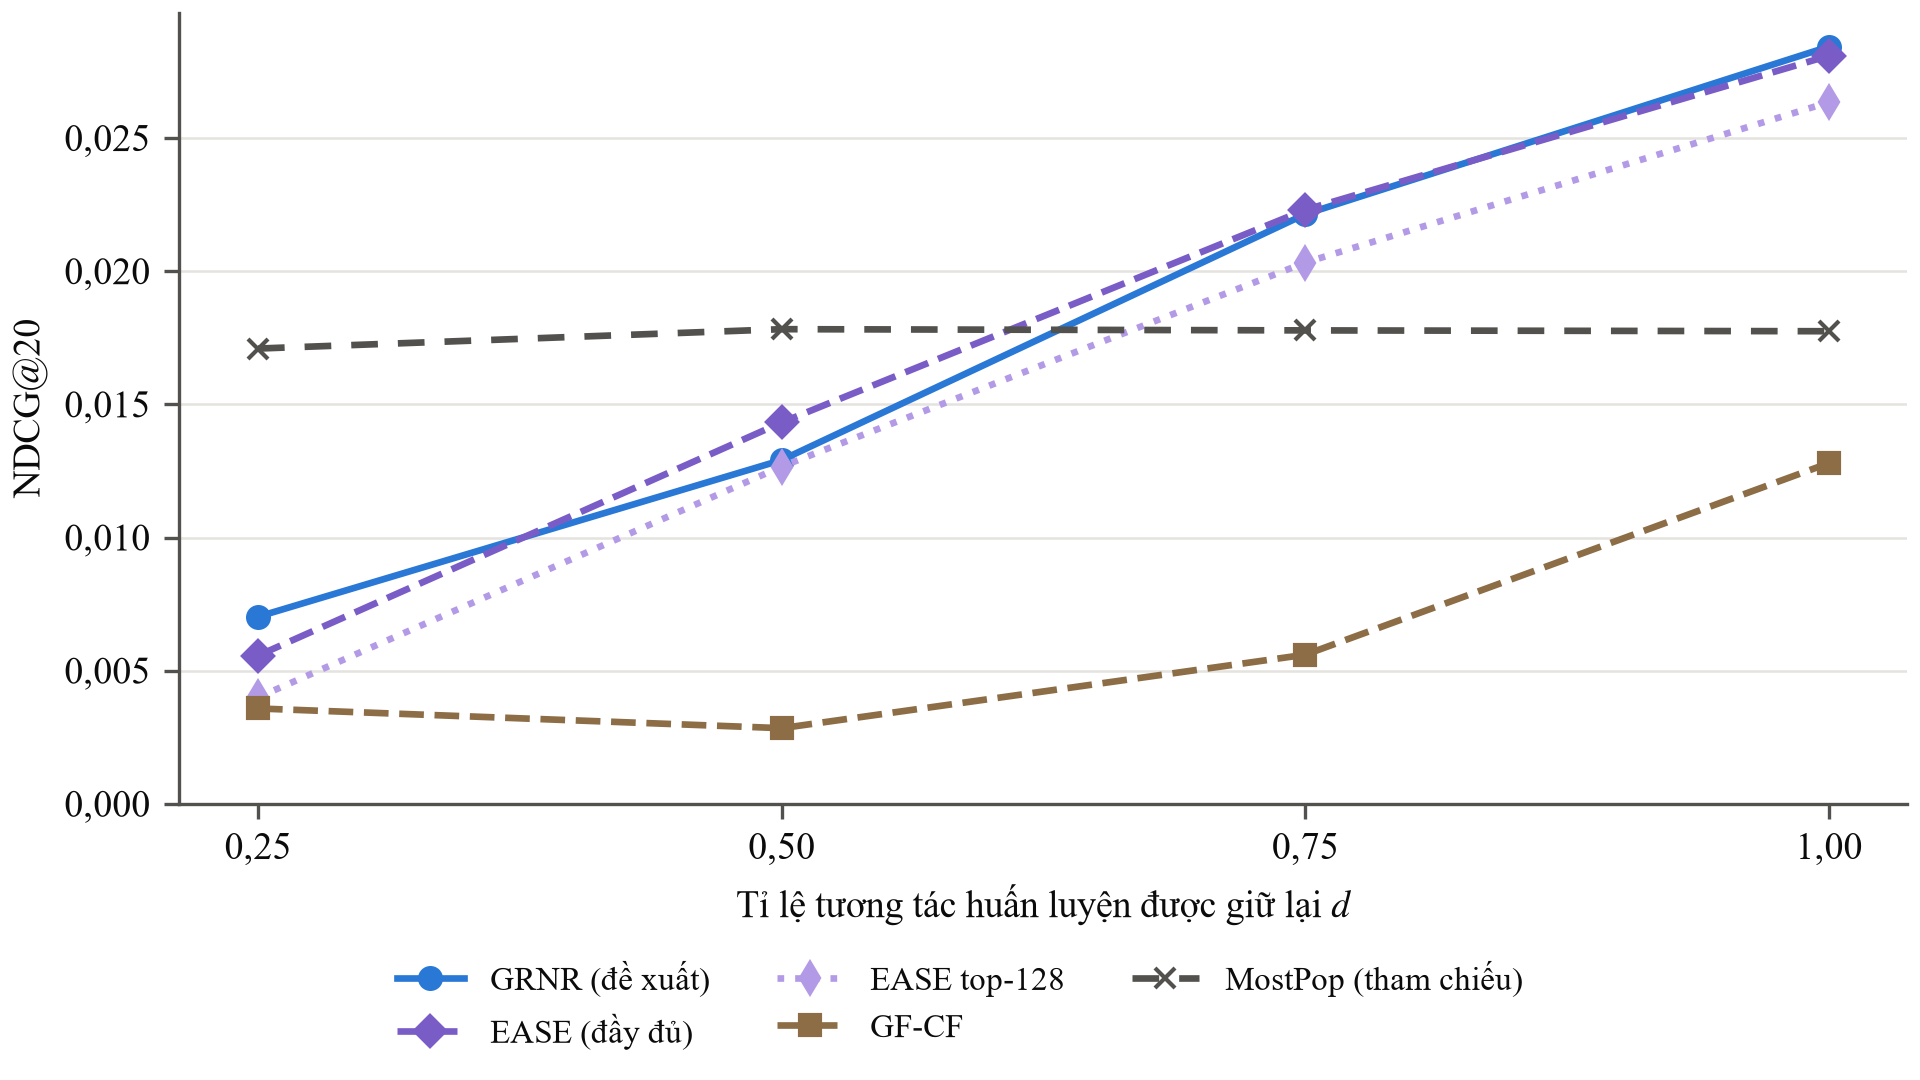
\includegraphics[width=\linewidth,height=0.67\textheight,keepaspectratio]{figures/fig_5_6_GRNR_vs_MostPop.png}
\takeaway{$d=0{,}5$: thấp hơn EASE đầy đủ (9,8\%). $d=0{,}25$: \textbf{cao hơn EASE đầy đủ 26,2\%} (KTC $\Delta$ trên 0), nhưng vẫn \textbf{thấp hơn MostPop 58,9\%}.}
\end{frame}

\begin{frame}{GRNR mất tín hiệu gì khi dữ liệu thưa?}
\centering
{\small\bfseries\color{PrimaryBlue}Chỉ giữ 25\% tương tác không có nghĩa giữ 25\% tín hiệu}\par
\vspace{0.09cm}

\begin{columns}[T,onlytextwidth]

\begin{column}{0.45\textwidth}
    \metric{4,2\%}{Cặp đồng xuất hiện còn lại}
\end{column}
\hfill
\begin{column}{0.45\textwidth}
    \metric{12,7\%}{Sản phẩm không còn láng giềng}
\end{column}

\end{columns}

\vspace{0.10cm}
\begin{tikzpicture}[
 left/.style={draw=PrimaryBlue,rounded corners=4pt,fill=PaleBlue,
 minimum height=1.03cm,text width=4.1cm,align=center,font=\small,inner sep=6pt},
 ar/.style={-Latex,line width=1.3pt,draw=PrimaryBlue}]
\node[left] (l) {\textbf{Có đồng xuất hiện}\\Sản phẩm trong cùng lịch sử};
\node[left,right=1.0cm of l] (r) {\textbf{Khi tín hiệu cạn}\\Ít láng giềng, trọng số khó ước lượng};
\draw[ar] (l) -- (r);
\end{tikzpicture}
\vspace{0.04cm}
\begin{block}{Hệ quả với GRNR (Bảng 5.4)}
\small Số láng giềng trung bình giảm từ \textbf{89,8} xuống \textbf{11,1}. Sản phẩm cô lập chỉ còn hệ số chặn $b_i$ trong điểm số.
\end{block}
\takeaway{Tín hiệu đồng xuất hiện suy giảm mạnh; cần ablation để xác định tác động riêng của $b_i$.}
\end{frame}

\begin{frame}{GRNR: Lợi thế dung lượng gần 190 lần}
\centering
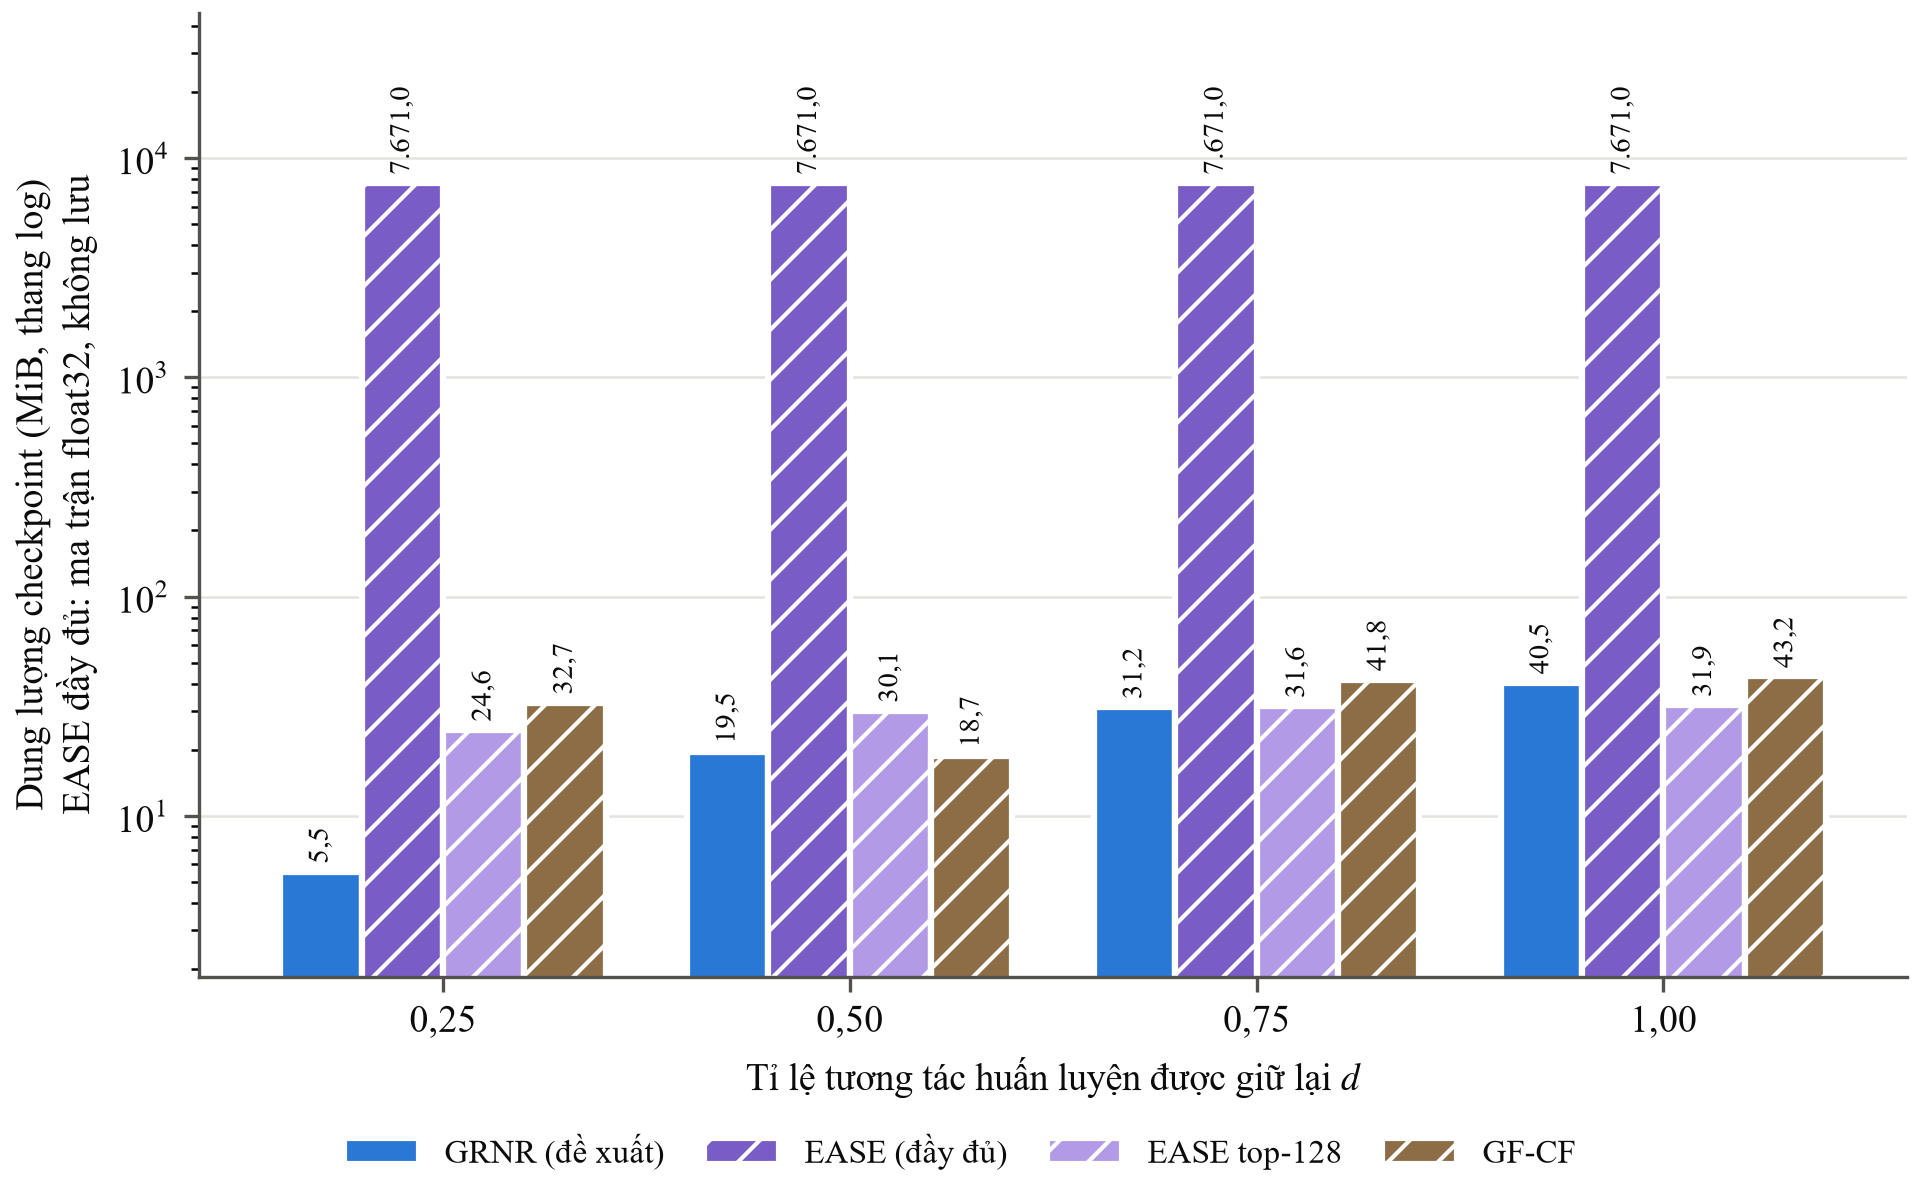
\includegraphics[width=\linewidth,height=0.60\textheight,keepaspectratio]{figures/fig_5_15_GRNR_Memory.png}
\vspace{0.04cm}
\begin{columns}[T,totalwidth=\textwidth]
\column{0.46\textwidth}
\begin{block}{\centering\large\bfseries 40,5 MiB}
\centering\footnotesize Checkpoint GRNR ($d=1$)
\end{block}
\column{0.46\textwidth}
\begin{block}{\centering\large\bfseries 7,5 GiB}
\centering\footnotesize Ma trận EASE đầy đủ (ước tính)
\end{block}
\end{columns}
\shortnote{GRNR nhỏ hơn xấp xỉ 190 lần; thời gian chạy giữa các thiết bị chỉ có ý nghĩa tham khảo.}
\end{frame}
